\documentclass{standalone}
\usepackage{tikz}
\usetikzlibrary{patterns, positioning}


\begin{document}
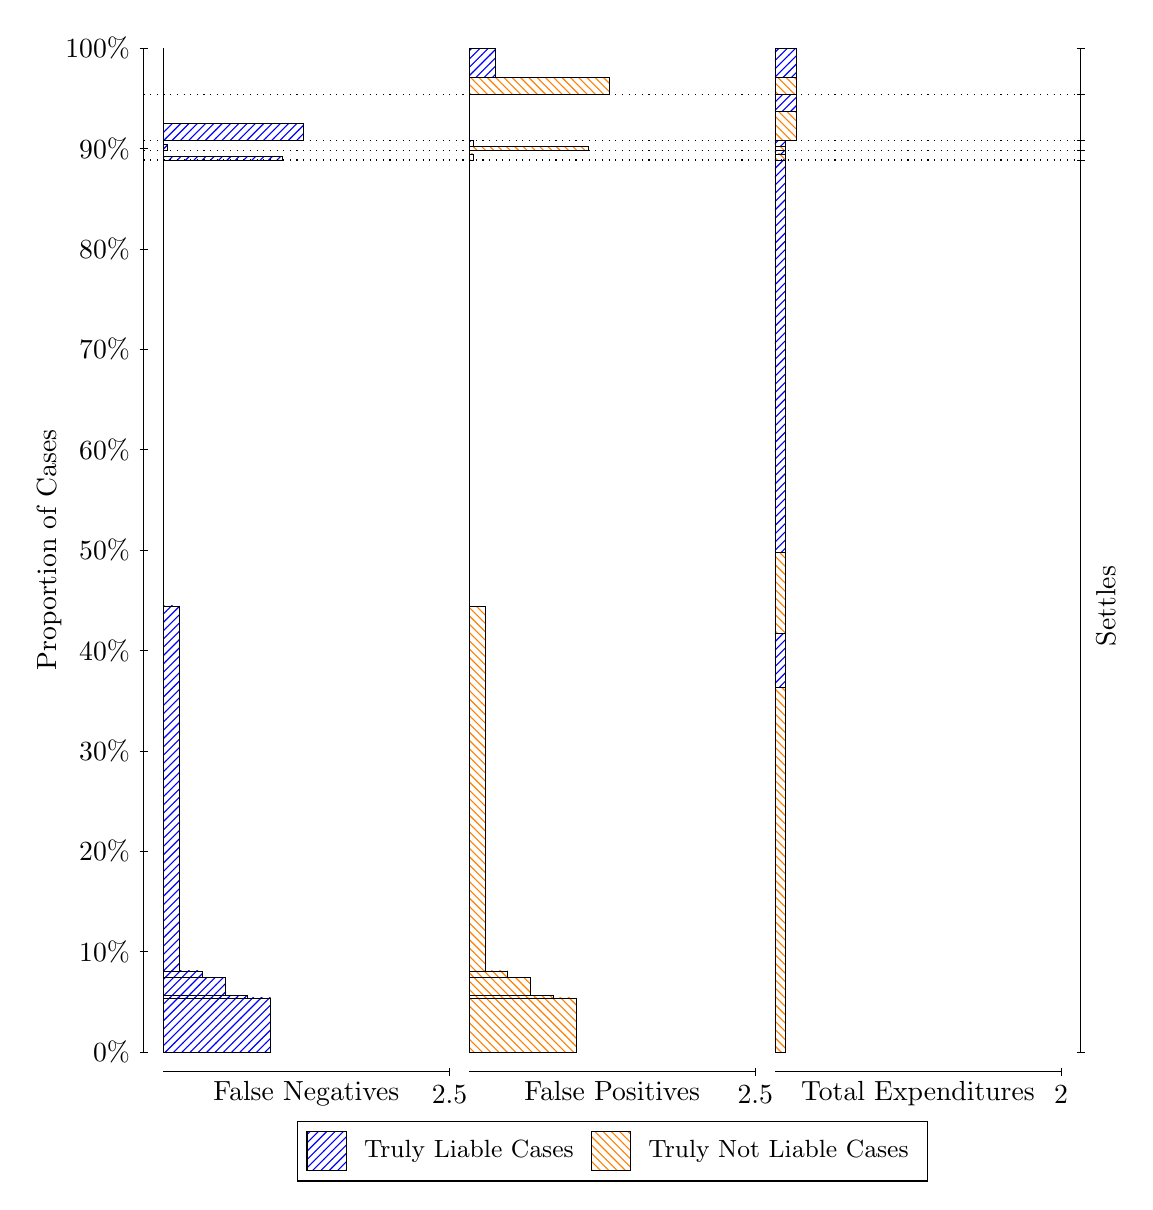
\begin{tikzpicture}
\draw[black, very thin] (1.5,1.75) -- (1.5,14.5);
\node[rotate=90, text=black, anchor=center] at (0.3, 8.125) {Proportion of Cases};
\draw[black, very thin] (1.45,1.75) -- (1.55,1.75);
\node[text=black, anchor=east] at (1.45, 1.75) {0\%};
\draw[black, very thin] (1.45,3.025) -- (1.55,3.025);
\node[text=black, anchor=east] at (1.45, 3.025) {10\%};
\draw[black, very thin] (1.45,4.3) -- (1.55,4.3);
\node[text=black, anchor=east] at (1.45, 4.3) {20\%};
\draw[black, very thin] (1.45,5.575) -- (1.55,5.575);
\node[text=black, anchor=east] at (1.45, 5.575) {30\%};
\draw[black, very thin] (1.45,6.85) -- (1.55,6.85);
\node[text=black, anchor=east] at (1.45, 6.85) {40\%};
\draw[black, very thin] (1.45,8.125) -- (1.55,8.125);
\node[text=black, anchor=east] at (1.45, 8.125) {50\%};
\draw[black, very thin] (1.45,9.4) -- (1.55,9.4);
\node[text=black, anchor=east] at (1.45, 9.4) {60\%};
\draw[black, very thin] (1.45,10.675) -- (1.55,10.675);
\node[text=black, anchor=east] at (1.45, 10.675) {70\%};
\draw[black, very thin] (1.45,11.95) -- (1.55,11.95);
\node[text=black, anchor=east] at (1.45, 11.95) {80\%};
\draw[black, very thin] (1.45,13.225) -- (1.55,13.225);
\node[text=black, anchor=east] at (1.45, 13.225) {90\%};
\draw[black, very thin] (1.45,14.5) -- (1.55,14.5);
\node[text=black, anchor=east] at (1.45, 14.5) {100\%};

\draw[black, very thin] (13.4,1.75) -- (13.4,14.5);
\draw[black, very thin] (13.35,1.75) -- (13.45,1.75);
\node[anchor=west] at (13.35, 1.75) {};
\draw[black, very thin] (13.35,13.078) -- (13.45,13.078);
\node[anchor=west] at (13.35, 13.078) {};
\draw[black, very thin] (13.35,13.204) -- (13.45,13.204);
\node[anchor=west] at (13.35, 13.204) {};
\draw[black, very thin] (13.35,13.33) -- (13.45,13.33);
\node[anchor=west] at (13.35, 13.33) {};
\draw[black, very thin] (13.35,13.915) -- (13.45,13.915);
\node[anchor=west] at (13.35, 13.915) {};
\draw[black, very thin] (13.35,14.5) -- (13.45,14.5);
\node[anchor=west] at (13.35, 14.5) {};

\draw[black, very thin, pattern color=blue, pattern=north east lines] (1.75,1.75) rectangle (3.1125,2.4357);
\draw[black, very thin, pattern color=blue, pattern=north east lines] (1.75,2.4357) rectangle (2.8218,2.4722);
\draw[black, very thin, pattern color=blue, pattern=north east lines] (1.75,2.4722) rectangle (2.5312,2.6971);
\draw[black, very thin, pattern color=blue, pattern=north east lines] (1.75,2.6971) rectangle (2.2405,2.7797);
\draw[black, very thin, pattern color=blue, pattern=north east lines] (1.75,2.7797) rectangle (1.9498,7.4139);
\draw[black, very thin, pattern color=orange, pattern=north west lines] (1.75,7.4139) rectangle (1.75,13.078);
\draw[black, very thin, pattern color=blue, pattern=north east lines] (1.75,13.078) rectangle (3.2578,13.126);
\draw[black, very thin, pattern color=orange, pattern=north west lines] (1.75,13.126) rectangle (1.75,13.204);
\draw[black, very thin, pattern color=blue, pattern=north east lines] (1.75,13.204) rectangle (1.8045,13.281);
\draw[black, very thin, pattern color=orange, pattern=north west lines] (1.75,13.281) rectangle (1.75,13.33);
\draw[black, very thin, pattern color=blue, pattern=north east lines] (1.75,13.33) rectangle (3.5303,13.547);
\draw[black, very thin, pattern color=orange, pattern=north west lines] (1.75,13.547) rectangle (1.75,13.915);
\draw[black, very thin, pattern color=orange, pattern=north west lines] (1.75,13.915) rectangle (1.75,14.132);
\draw[black, very thin, pattern color=blue, pattern=north east lines] (1.75,14.132) rectangle (1.75,14.5);
\draw[black, very thin, pattern color=orange, pattern=north west lines] (5.6333,1.75) rectangle (6.9958,2.4357);
\draw[black, very thin, pattern color=orange, pattern=north west lines] (5.6333,2.4357) rectangle (6.7052,2.4722);
\draw[black, very thin, pattern color=orange, pattern=north west lines] (5.6333,2.4722) rectangle (6.4145,2.6971);
\draw[black, very thin, pattern color=orange, pattern=north west lines] (5.6333,2.6971) rectangle (6.1238,2.7797);
\draw[black, very thin, pattern color=orange, pattern=north west lines] (5.6333,2.7797) rectangle (5.8332,7.4138);
\draw[black, very thin, pattern color=blue, pattern=north east lines] (5.6333,7.4138) rectangle (5.6333,13.078);
\draw[black, very thin, pattern color=orange, pattern=north west lines] (5.6333,13.078) rectangle (5.6878,13.155);
\draw[black, very thin, pattern color=blue, pattern=north east lines] (5.6333,13.155) rectangle (5.6333,13.204);
\draw[black, very thin, pattern color=orange, pattern=north west lines] (5.6333,13.204) rectangle (7.1412,13.252);
\draw[black, very thin, pattern color=blue, pattern=north east lines] (5.6333,13.252) rectangle (5.6878,13.33);
\draw[black, very thin, pattern color=orange, pattern=north west lines] (5.6333,13.33) rectangle (5.6333,13.698);
\draw[black, very thin, pattern color=blue, pattern=north east lines] (5.6333,13.698) rectangle (5.6333,13.915);
\draw[black, very thin, pattern color=orange, pattern=north west lines] (5.6333,13.915) rectangle (7.4137,14.132);
\draw[black, very thin, pattern color=blue, pattern=north east lines] (5.6333,14.132) rectangle (5.9603,14.5);
\draw[black, very thin, pattern color=orange, pattern=north west lines] (9.5167,1.75) rectangle (9.6529,6.384);
\draw[black, very thin, pattern color=blue, pattern=north east lines] (9.5167,6.384) rectangle (9.6529,7.0698);
\draw[black, very thin, pattern color=orange, pattern=north west lines] (9.5167,7.0698) rectangle (9.6529,8.0995);
\draw[black, very thin, pattern color=blue, pattern=north east lines] (9.5167,8.0995) rectangle (9.6529,13.078);
\draw[black, very thin, pattern color=orange, pattern=north west lines] (9.5167,13.078) rectangle (9.6529,13.155);
\draw[black, very thin, pattern color=blue, pattern=north east lines] (9.5167,13.155) rectangle (9.6529,13.204);
\draw[black, very thin, pattern color=orange, pattern=north west lines] (9.5167,13.204) rectangle (9.6529,13.252);
\draw[black, very thin, pattern color=blue, pattern=north east lines] (9.5167,13.252) rectangle (9.6529,13.33);
\draw[black, very thin, pattern color=orange, pattern=north west lines] (9.5167,13.33) rectangle (9.7892,13.698);
\draw[black, very thin, pattern color=blue, pattern=north east lines] (9.5167,13.698) rectangle (9.7892,13.915);
\draw[black, very thin, pattern color=orange, pattern=north west lines] (9.5167,13.915) rectangle (9.7892,14.132);
\draw[black, very thin, pattern color=blue, pattern=north east lines] (9.5167,14.132) rectangle (9.7892,14.5);
\draw[black, dotted] (1.5,13.078) -- (13.4,13.078);
\draw[black, dotted] (1.5,13.204) -- (13.4,13.204);
\draw[black, dotted] (1.5,13.33) -- (13.4,13.33);
\draw[black, dotted] (1.5,13.915) -- (13.4,13.915);
\draw[black, very thin] (1.75,1.5) -- (5.3833,1.5);
\node[text=black, anchor=north] at (3.5667, 1.5) {False Negatives};
\draw[black, very thin] (5.3833,1.45) -- (5.3833,1.55);
\node[text=black, anchor=north] at (5.3833, 1.45) {2.5};

\draw[black, very thin] (5.6333,1.5) -- (9.2667,1.5);
\node[text=black, anchor=north] at (7.45, 1.5) {False Positives};
\draw[black, very thin] (9.2667,1.45) -- (9.2667,1.55);
\node[text=black, anchor=north] at (9.2667, 1.45) {2.5};

\draw[black, very thin] (9.5167,1.5) -- (13.15,1.5);
\node[text=black, anchor=north] at (11.333, 1.5) {Total Expenditures};
\draw[black, very thin] (13.15,1.45) -- (13.15,1.55);
\node[text=black, anchor=north] at (13.15, 1.45) {2};

\node[text=black, centered, rotate=90] at (13.72, 7.4138) {Settles};





\draw (7.449999999999999,1.5) node[draw=none] (baseCoordinate) {};
\begin{scope}[align=center]
        \matrix[scale=0.5, draw=black, below=0.5cm of baseCoordinate, nodes={draw}, column sep=0.1cm]{
            \node[rectangle, draw, minimum width=0.5cm, minimum height=0.5cm, pattern color=blue, pattern=north east lines] {}; &
            \node[draw=none, font=\small, text=black] (B) {Truly Liable Cases}; &
            \node[rectangle, draw, minimum width=0.5cm, minimum height=0.5cm, pattern color=orange, pattern=north west lines] {}; &
            \node[draw=none, font=\small, text=black] (B) {Truly Not Liable Cases}; \\
            };
\end{scope}

\end{tikzpicture}
\end{document}